%% $Id: nested_grids.tex,v 1.5 2006/02/21 16:58:01 benkirk Exp $
\chapter{Nested Grids\label{chap:nested_grids}}
%\newcommand{\bdoc}{\begin{document}}
%\newcommand{\edoc}{\end{document}}
%\newcommand{\ben}{\begin{enumerate}}
%\newcommand{\een}{\end{enumerate}}
%\newcommand{\binit}{\begin{itemize}}
%\newcommand{\eit}{\end{itemize}}
%\newcommand{\bdes}{\begin{description}}
%\newcommand{\edes}{\end{description}}
%\newcommand{\bc}{\begin{center}}
%\newcommand{\ec}{\end{center}}
%\newcommand{\bflt}{\begin{flushleft}}
%\newcommand{\eflt}{\end{flushleft}}
%\newcommand{\bfrt}{\begin{flushright}}
%\newcommand{\efrt}{\end{flushright}}
%\newcommand{\be}{\begin{equation}}
%\newcommand{\ee}{\end{equation}}
%\newcommand{\bes}{\begin{displaymath}}
%\newcommand{\ees}{\end{displaymath}}
%\newcommand{\ba}{\begin{array}}
%\newcommand{\ea}{\end{array}}
%\newcommand{\bea}{\begin{eqnarray}}
%\newcommand{\eea}{\end{eqnarray}}
%\newcommand{\beas}{\begin{eqnarray*}}
%\newcommand{\eeas}{\end{eqnarray*}}
%\newcommand{\np}{\newpage}
%\newcommand{\bsni}{\bigskip \noindent}
%\newcommand{\nn}{\nonumber}
%\newcommand{\ds}{\displaystyle}
%\newcommand{\ts}{\textstyle}
%\newcommand{\sstyle}{\scriptstyle}
%\newcommand{\ssstyle}{\scriptscriptstyle}
%%
%\newcommand{\Dt}{\mbox{${\Delta t}$}}
%\newcommand{\Dx}{\mbox{${\Delta x}$}}
%%
%\newcommand{\bfa}{\mbox{\boldmath $a$}}
\newcommand{\bfb}{\mbox{\boldmath $b$}}
%\newcommand{\bfc}{\mbox{\boldmath $c$}}
%\newcommand{\bfd}{\mbox{\boldmath $d$}}
%\newcommand{\bfe}{\mbox{\boldmath $e$}}
\newcommand{\bff}{\mbox{\boldmath $f$}}
\newcommand{\bfg}{\mbox{\boldmath $g$}}
%\newcommand{\bfh}{\mbox{\boldmath $h$}}
%\newcommand{\bfi}{\mbox{\boldmath $i$}}
%\newcommand{\bfj}{\mbox{\boldmath $j$}}
%\newcommand{\bfk}{\mbox{\boldmath $k$}}
%\newcommand{\bfl}{\mbox{\boldmath $l$}}
%\newcommand{\bfm}{\mbox{\boldmath $m$}}
%\newcommand{\bfn}{\mbox{\boldmath $n$}}
%\newcommand{\bfo}{\mbox{\boldmath $o$}}
\newcommand{\bfp}{\mbox{\boldmath $p$}}
%\newcommand{\bfq}{\mbox{\boldmath $q$}}
%\newcommand{\bfr}{\mbox{\boldmath $r$}}
\newcommand{\bfs}{\mbox{\boldmath $s$}}
%\newcommand{\bft}{\mbox{\boldmath $t$}}
\newcommand{\bfu}{\mbox{\boldmath $u$}}
\newcommand{\bfv}{\mbox{\boldmath $v$}}
\newcommand{\bfw}{\mbox{\boldmath $w$}}
%\newcommand{\bfx}{\mbox{\boldmath $x$}}
%\newcommand{\bfy}{\mbox{\boldmath $y$}}
%\newcommand{\bfz}{\mbox{\boldmath $z$}}
%%
\newcommand{\bfA}{\mbox{\boldmath $A$}}
\newcommand{\bfB}{\mbox{\boldmath $B$}}
\newcommand{\bfC}{\mbox{\boldmath $C$}}
\newcommand{\bfD}{\mbox{\boldmath $D$}}
%\newcommand{\bfE}{\mbox{\boldmath $E$}}
\newcommand{\bfF}{\mbox{\boldmath $F$}}
\newcommand{\bfG}{\mbox{\boldmath $G$}}
\newcommand{\bfH}{\mbox{\boldmath $H$}}
%\newcommand{\bfI}{\mbox{\boldmath $I$}}
%\newcommand{\bfJ}{\mbox{\boldmath $J$}}
\newcommand{\bfK}{\mbox{\boldmath $K$}}
%\newcommand{\bfL}{\mbox{\boldmath $L$}}
\newcommand{\bfM}{\mbox{\boldmath $M$}}
%\newcommand{\bfN}{\mbox{\boldmath $N$}}
%\newcommand{\bfO}{\mbox{\boldmath $O$}}
%\newcommand{\bfP}{\mbox{\boldmath $P$}}
\newcommand{\bfQ}{\mbox{\boldmath $Q$}}
%\newcommand{\bfR}{\mbox{\boldmath $R$}}
\newcommand{\bfS}{\mbox{\boldmath $S$}}
\newcommand{\bfT}{\mbox{\boldmath $T$}}
\newcommand{\bfU}{\mbox{\boldmath $U$}}
%\newcommand{\bfV}{\mbox{\boldmath $V$}}
%\newcommand{\bfW}{\mbox{\boldmath $W$}}
%\newcommand{\bfX}{\mbox{\boldmath $X$}}
%\newcommand{\bfY}{\mbox{\boldmath $Y$}}
%\newcommand{\bfZ}{\mbox{\boldmath $Z$}}
%%
%\newcommand{\alp}{{\alpha}}
%\newcommand{\bet}{{\beta}}
%\newcommand{\gam}{{\gamma}}
%\newcommand{\del}{{\delta}}
%\newcommand{\eps}{{\epsilon}}
%\newcommand{\vareps}{{\varepsilon}}
%\newcommand{\zet}{{\zeta}}
%\newcommand{\thet}{{\theta}}
%\newcommand{\varthet}{\vartheta}
%\newcommand{\iot}{{\iota}}
%\newcommand{\kap}{{\kappa}}
%\newcommand{\lam}{{\lambda}}
%\newcommand{\sig}{{\sigma}}
%\newcommand{\ups}{{\upsilon}}
%\newcommand{\ome}{{\omega}}
%%
%\newcommand{\Gam}{{\Gamma}}
%\newcommand{\Del}{{\Delta}}
%\newcommand{\Thet}{{\Theta}}
%\newcommand{\Lam}{{\Lambda}}
%\newcommand{\Sig}{{\Sigma}}
%\newcommand{\Ups}{{\Upsilon}}
%\newcommand{\Ome}{{\Omega}}
%%
%\newcommand{\bfalp}{\mbox{\boldmath $\alpha$}}
%\newcommand{\bfbet}{\mbox{\boldmath $\beta$}}
%\newcommand{\bfgam}{\mbox{\boldmath $\gamma$}}
%\newcommand{\bfdel}{\mbox{\boldmath $\delta$}}
%\newcommand{\bfeps}{\mbox{\boldmath $\epsilon$}}
%\newcommand{\bfvareps}{\mbox{\boldmath $\varepsilon$}}
%\newcommand{\bfzet}{\mbox{\boldmath $\zeta$}}
%\newcommand{\bfeta}{\mbox{\boldmath $\eta$}}
%\newcommand{\bfthet}{\mbox{\boldmath $\theta$}}
%\newcommand{\bfiot}{\mbox{\boldmath $\iota$}}
%\newcommand{\bfkap}{\mbox{\boldmath $\kappa$}}
%\newcommand{\bflam}{\mbox{\boldmath $\lambda$}}
%\newcommand{\bfmu}{\mbox{\boldmath $\mu$}}
%\newcommand{\bfnu}{\mbox{\boldmath $\nu$}}
%\newcommand{\bfxi}{\mbox{\boldmath $\xi$}}
%\newcommand{\bfpi}{\mbox{\boldmath $\pi$}}
%\newcommand{\bfrho}{\mbox{\boldmath $\rho$}}
%\newcommand{\bfsig}{\mbox{\boldmath $\sigma$}}
\newcommand{\bftau}{\mbox{\boldmath $\tau$}}
%\newcommand{\bfups}{\mbox{\boldmath $\upsilon$}}
%\newcommand{\bfphi}{\mbox{\boldmath $\phi$}}
%\newcommand{\bfchi}{\mbox{\boldmath $\chi$}}
%\newcommand{\bfpsi}{\mbox{\boldmath $\psi$}}
%\newcommand{\bfome}{\mbox{\boldmath $\omega$}}
%%
%\newcommand{\bfGam}{\mbox{\boldmath $\Gamma$}}
%\newcommand{\bfDel}{\mbox{\boldmath $\Delta$}}
%\newcommand{\bfThet}{\mbox{\boldmath $\Theta$}}
%\newcommand{\bfLam}{\mbox{\boldmath $\Lambda$}}
%\newcommand{\bfXi}{\mbox{\boldmath $\Xi$}}
%\newcommand{\bfPi}{\mbox{\boldmath $\Pi$}}
%\newcommand{\bfSig}{\mbox{\boldmath $\Sigma$}}
%\newcommand{\bfUps}{\mbox{\boldmath $\Upsilon$}}
%\newcommand{\bfPhi}{\mbox{\boldmath $\Phi$}}
%\newcommand{\bfPsi}{\mbox{\boldmath $\Psi$}}
%\newcommand{\bfOme}{\mbox{\boldmath $\Omega$}}
%%
%\newcommand{\ptl}{{\partial}}
%\newcommand{\nab}{{\nabla}}
%%
%\newcommand{\bfptl}{\mbox{\boldmath $\partial$}}
%\newcommand{\bfnab}{\mbox{\boldmath $\nabla$}}
%\newcommand{\bfinfty}{\mbox{\boldmath $\infty$}}
%\newcommand{\bfto}{\mbox{\boldmath $\to$}}
%\newcommand{\bfimath}{\mbox{\boldmath $\imath$}}
%\newcommand{\bfjmath}{\mbox{\boldmath $\jmath$}}
%\newcommand{\bfsum}{\mbox{\boldmath $\sum$}}
%%
%\newcommand{\calA}{\mbox{${\cal A}$}}
%\newcommand{\calB}{\mbox{${\cal B}$}}
%\newcommand{\calC}{\mbox{${\cal C}$}}
%\newcommand{\calD}{\mbox{${\cal D}$}}
%\newcommand{\calE}{\mbox{${\cal E}$}}
%\newcommand{\calF}{\mbox{${\cal F}$}}
%\newcommand{\calG}{\mbox{${\cal G}$}}
%\newcommand{\calH}{\mbox{${\cal H}$}}
%\newcommand{\calI}{\mbox{${\cal I}$}}
%\newcommand{\calJ}{\mbox{${\cal J}$}}
%\newcommand{\calK}{\mbox{${\cal K}$}}
%\newcommand{\calL}{\mbox{${\cal L}$}}
%\newcommand{\calM}{\mbox{${\cal M}$}}
%\newcommand{\calN}{\mbox{${\cal N}$}}
%\newcommand{\calO}{\mbox{${\cal O}$}}
%\newcommand{\calP}{\mbox{${\cal P}$}}
%\newcommand{\calQ}{\mbox{${\cal Q}$}}
%\newcommand{\calR}{\mbox{${\cal R}$}}
%\newcommand{\calS}{\mbox{${\cal S}$}}
%\newcommand{\calT}{\mbox{${\cal T}$}}
%\newcommand{\calU}{\mbox{${\cal U}$}}
%\newcommand{\calV}{\mbox{${\cal V}$}}
%\newcommand{\calW}{\mbox{${\cal W}$}}
%\newcommand{\calX}{\mbox{${\cal X}$}}
%\newcommand{\calY}{\mbox{${\cal Y}$}}
%\newcommand{\calZ}{\mbox{${\cal Z}$}}
%%
%\newcommand{\degrees}{\mbox{$^\circ$}}
%\newcommand{\pdv}[2]{\frac{\partial{#1}}{\partial{#2}}}
%\newcommand{\dv}[2]{\frac{d{#1}}{d{#2}}}
%\newcommand{\intgl}[2]{\ds \int^{#1}_{#2}}
%\newcommand{\sums}[2]{\ds \sum^{#1}_{#2}}
%\newcommand{\dsfrac}[2]{\ds \frac{#1}{#2}}
%\newcommand{\tsfrac}[2]{\ts \frac{#1}{#2}}
%\newcommand{\ldb}{\ [\![\ }
%\newcommand{\rdb}{\ ]\!]\ } 
%\newcommand{\ia}{\int\!\!\!\int\limits_{\!\!\!\!\rm Area}}
%\newcommand{\RR}{R\!\!\!\!R}
%\newcommand{\fR}{\mbox{I}\!\mbox{R}}
%\newcommand{\fC}{\mbox{I}\!\!\!\!\!\;\mbox{C}}
%\newcommand{\vbar}{\vee \!\!\!\!\!\! -}
%\newcommand{\wh}{\widehat}



\def\p{{\partial}}
\def\cI{{\cal I}}
\def\cP{{\cal P}}
\def\fnorm{{\| f \|_0}}

\def\Frac{\displaystyle \frac}

\def\cA{{\cal A}}
\def\dt{\Delta t}
\def\cA{{\bf {\cal A}}}

\def\bu{\mbox{{\boldmath $u$}}}
\def\bF{\mbox{{\boldmath $f$}}}


%%%%%%%%%%%%%%%%%%%%%%%%%%%%%%%%%%%%%%%%%%%%%%%%%%%%%%%%%%%
\section{Introduction}
In this study we investigate the use of nested grid
iteration, or cascadic multigrid (CMG) as it is sometimes
termed, to solve viscous flow and transport problems.  Of particular
interest are large scale finite element or analogous finite volume
and finite difference simulations on distributed parallel computer
systems.

The basic idea in the CMG approach is simply to smooth the
solution iterate on successively refined grids.  This type of nested
iteration scheme has been previously applied to accelerate
convergence~\cite{CarHum81}. It may also be used in conjunction with
other continuation processes.  For example, one can apply incremental
continuation in a parameter such as the applied load, source strength,
Reynolds number, or Rayleigh number while simultaneously applying
cascadic continuation from coarse to fine grids.  The main attributes
of the approach are its simplicity and the fact that it can be easily
incorporated into existing simulation codes.  This
is an important consideration as we recognize the additional
complexity of simulation algorithms and codes needed for coupled
multiphysics simulations and the need to accommodate multiple scales
through mesh refinement.  Moreover, requirements for distributed
parallel simulation and the need to include local adaptive mesh
refinement are additional incentives.  At the same time, it is
important to recognize that CMG will not deliver the optimal
preconditioning properties of full multigrid, V-cycle multigrid, and
high quality subdomain preconditioners.

The primary class of applications suitable for this approach
correspond to steady state linear and nonlinear elliptic boundary
value problems (although the method may also be beneficial for implicit
time integration schemes applied to unsteady processes).  For example, the
approach has been used successfully
for nonlinear adaptive mesh refinement simulations as described  in~\cite{carey_gridbook}.
In one such test case it is shown that a single Newton solve per nested mesh
iteration is computationally very  efficient compared with alternative
strategies that involved iteration to a finer tolerance on intermediate
meshes.  In other cases it is
shown that the standard Newton method fails to converge if it is
applied to the optimal graded mesh whereas application on nested
meshes with parameter continuation converges.  Clearly, most adaptive
mesh refinement (AMR) schemes exploit this idea in some form.

The approach has been applied to  plane elasticity problems \cite{ShaGil96}, the Stokes equations \cite{BraDah99}, and the plate bending problem \cite{ShiXu98}. Convergence has been studied for non-conforming finite elements in \cite{Ste98} and mortar finite elements in \cite{braess-2002-subspace}. Recently,  application to parabolic problems has been considered in \cite{ShiXu99}. Our main purpose here is to investigate the scheme for
solution of stationary and transient incompressible viscous flow and
transport problems and to consider some related issues.  We
consider the primitive variable (velocity/pressure) formulation with
finite element approximation using consistent spaces (satisfying the
LBB or inf-sup condition).  In the 3-D applications we use
tri--quadratic approximation of the velocity and tri--linear
approximation of the pressure on hexahedral elements.  For the heat
and species transport equations we employ the tri--quadratic element basis
for each scalar field variable. The CMG approach is applied in
conjunction with representative Krylov subspace iterative solution of
the linear systems on each mesh. More specifically, a bi-conjugate gradient solution of
the Jacobian subsystems for Newton iteration is carried out on each
mesh along the CMG refinement path.  In the present work the
numerical experiments will be confined to uniformly nested grids.

Parallelization of the problem is carried out by partitioning
to processor subdomains~\cite{carey_world_scientific_2000} and in the present case the uniform
CMG scheme clearly implies that an initial well-balanced partition
will remain so.  Hence, in this restricted setting, an investment in an
initial high quality partitioning by means of a spectral algorithm or
multilevel Kernigan Lin  algorithm easily is justified.  In the case of AMR in parallel
 there will obviously be a need for dynamic
repartitioning to balance the load~\cite{ZoltanOverviewArticle}.

The outline of the present treatment is as follows:  In the
next section we introduce the CMG scheme for a representative
elliptic boundary value problem and summarize the main underlying
error estimates, desired smoothing properties and arithmetic
complexity under these assumptions.  Then in Section~\ref{governing_equations}
we give the
governing equations for the coupled viscous flow and transport
problems of interest in the present applications study.  The
approximate formulation is also stated and the Newton BCG algorithm
is outlined.  (The 2D simulation studies are similarly based, but additional Krylov solvers such as
BCG--Stab and GMRES are available for serial computations). The zero diagonal
block in the resulting matrix for the saddle point problem poses some
difficulties and in Section~\ref{precond} we describe a strategy for selecting a
diagonal perturbation for the preconditioner.  Next, in
Section~\ref{numerical_experiments} we provide the results of serial and parallel numerical
experiments in three categories:  (i) comparison studies of CMG using
different diagonal treatments for the pressure;  (ii) performance
studies of CMG for 3D linear Stokes flow and low Reynolds number Navier
Stokes flow in parallel; (iii) 2D Navier Stokes flow examining the influence of different iterative solvers on the performance of the CMG algorithm.


%%%%%%%%%%%%%%%%%%%%%%%%%%%%%%%%%%%%%%%%%%%%%%%%%%%%%%%%%%%
\section{Classical cascadic multigrid method\label{cmg_theory}}

In this section we describe a ``one-way'' multigrid method that
does not require a coarse grid correction. It is based on
the well known idea of iterative improvement on successively refined
meshes
(e.g. see \cite{Wac66}). More recently
there have been further theoretical studies of the mathematical
convergence
properties of this scheme and application to several areas. In
particular, Deuflhard and Bornemann \cite{Deu94,BD96} have made studies of
the
method which they refer to as a  cascadic multigrid algorithm and showed
that
an optimal iterative method with respect to the energy norm may be
obtained if conforming elements are used. To describe the basic ideas
of the cascadic multigrid method, we consider a simple elliptic boundary
value problem
\begin{equation}
  \label{simpleProblem}
  \begin{array}{rcll}
    -\Delta u &=& f & \mbox{~~in~~} ~~\Omega \\[.1ex]
    u &=& 0 & \mbox{~~on~~} \p\Omega
  \end{array}
\end{equation}
where $\Omega$ is a bounded Lipschitz domain in $\Re^d$, $d=2,3$.
For convenience let us also assume that the data are well behaved so
that
$u \in H^2_0(\Omega)$. (Problems with less
elliptic regularity ($u\in H^{1+\alpha}_0(\Omega)$, $0< \alpha< 1$)
are considered in \cite{BD96}.) The variational formulation of the
problem
is to find $u \in H^1_0(\Omega)$ such that
\begin{equation}
     \label{simpleVariational}
        a(u,\, v) = (f,\, v) \qquad \forall v \in H^1_0(\Omega)
\end{equation}
where $a(u,\, v) = \int\limits_{\Omega} \nabla u \cdot \nabla v \dx$ and
$(f,\, v) = \int\limits_{\Omega} f v\dx$. Hereafter
$\| u \|_a$ denotes the energy norm of $u$, $\| u \|_a^2 \equiv a(u,\,
u)$,
$\| u \|_1$ the $H^1$-norm and $\| u \|_0$ the $L_2$-norm. Note that
for the solution of problem (\ref{simpleVariational}) the energy norm is
equivalent
to the $H^1$-norm.

For the cascadic multigrid method we are interested in progressive
development of a fine grid solution to the steady state problem through
a
sequence of successively finer resolution grids and corresponding
finite
element approximations of (\ref{simpleVariational}). For convenience,
let
us take a sequence of nested  quasi-uniform fully
hierarchical grids $\Omega_j^h$, $0\le j \le L$. They generate a
sequence of finite element spaces $V_j$ such that
$$
V_0 \subset V_1 \subset \ldots \subset V_L \subset H^1_0(\Omega)
$$
where index $0$ is associated with a coarse grid and $L$ is the
number of grid refinements.

The definition of the multilevel procedure requires some additional
notations. For refinement levels $j=0,1,\ldots,L$, $u_j^h \in V_j$ are
finite element approximations given by
\begin{equation}
     \label{simpleDiscrete}
        a(u_j^h,\, v_j^h) = (f,\, v_j^h) \qquad \forall v_j^h \in V_j.
\end{equation}
Let $h_j$, $0\le j \le L$, denote an average size for the mesh elements
in
$\Omega_j^h$. For uniformly
nested grids, the relation $h_j \approx 2^{k-j} h_k$ is appropriate.
Finally, we let $u_j^*$ denote an approximate solution of
(\ref{simpleDiscrete}). Typically, after a coarse level direct solve,
the
approximate solution at subsequent higher levels is obtained by an
iterative scheme applied to (\ref{simpleDiscrete}). The idea is simply
to
solve the problem to a specified tolerance in the iterative scheme at a
given mesh level and then project the solution to a higher level as a
new
starting iterate. This process is repeated recursively through to the
final
mesh level.
The cascadic multigrid algorithm
may be summarized as follows:\vspace*{2mm}

\noindent
{\it
   \begin{tabular}{llp{80mm}}
     {\bf Cascadic MG:} & $j=0$ : &  $u_0^h \equiv u_j^*$ \\
                        &         &  direct solution of
                        (\ref{simpleDiscrete}) on the coarse
grid\\[0.9ex]
%
                        &$j=1,\ldots, L$ : & $u_j^0=\cP_j u_{j-1}^*$\\
                        &         & projection/interpolation to the finer grid
\\[.9ex]
%
                        &         & $u_j^*=\cI_j(m_j) u_{j}^0$\\
                        &         & iterative solution of problems
                        (\ref{simpleDiscrete}) on successively finer
                        grids \\[1.9ex]
   \end{tabular}\\
}
Here $\cP_j\colon V_{j-1} \to V_j$ is usually an interpolation operator, but other projections may be advantageous~\cite{CarSea85}.
$\cI_j(m_j)$ denotes $m_j$ steps of the basic iterative scheme
applied on level $j$. In the case of conforming finite elements, the
simplest choice for $\cP_j$ is the identity operator, i.e.
the initial guess for the iterative scheme is
the interpolated finite element solution from the previous level.

For the analysis of the cascadic multigrid algorithm the following
results from basic approximation theory \cite{Cia78} are used:
\begin{equation}
     \label{approximationProperties}
     \begin{array}{rcl}
         \| u - u_j^h \|_a  &\le&  c h_j \fnorm \\[.5ex]
         \| u_j^h - u_{j-1}^h \|_0  &\le&  c h_j \| u_j^h -
u_{j-1}^h\|_a,
         \quad 1 \le j \le L.
     \end{array}
\end{equation}

There are several possibilities for choosing a basic iterative scheme
(smoother) that are appropriate.
These include symmetric Gauss-Seidel (symGS), SSOR,
damped Jacobi (wJacobi) and the conjugate gradient (CG) or similar
Krylov
subspace  methods.
The error propagation on level $j$ is given by
$$
u_j^h - \cI_j(m_j) u_{j}^0 = S_j(m_j) (u_j^h - u_{j}^0)
$$
where mapping $S_j(m_j)\colon V_j \to V_j$ is assumed to have two
important smoothing properties:
\begin{equation}
  \label{smoothingProperties}
  \begin{array}{rcl}
    \| S_j(m_j) v_j^h \|_a  &\le&
    c \displaystyle\frac{h_j^{-1}}{m_j^\gamma} \| v_j^h\|_0
    \\[1.2ex]
    \| S_j(m_j) v_j^h \|_a  &\le& \| v_j^h \|_a, \qquad
    \forall v_j^h \in V_j,
  \end{array}
\end{equation}
with parameter $0 < \gamma \le 1$. In the energy norm such a
smoothing iteration reduces high frequency errors with $h$-independent
rate whereas low frequency error components are handled increasingly less
efficient for smaller and smaller $h$. 
The cascadic MG method is designed to handle low frequency error better. 
The three linear point iterative
schemes mentioned above satisfy (\ref{smoothingProperties})
with $\gamma = 1/2$ \cite{Hac85}. For the CG method we have better smoothing
properties with $\gamma = 1$ \cite{Sha96}. 

Note that the estimate (\ref{smoothingProperties}) is not the best 
one known for the CG method. Nevertheless it is sufficient to  
formulate the main convergence estimate for the cascadic MG method 
(see \cite{BD96,Sha96} for the proof).\vspace*{2mm}

{\it
  \noindent
      {\bf Theorem 1.} The error of the cascadic MG method with a smoother satisfying
      (\ref{smoothingProperties}) may be estimated by
      $$
      \| u_L^h - u_L^* \|_a \le c \sum\limits_{j=1}^L \frac{1}{m_j^\gamma}
      \| u_j^h - u_{j-1}^h \|_a \le
      c \left( \sum\limits_{j=1}^L \frac{h_j}{m_j^\gamma} \right) \fnorm.
      $$
}\vspace*{2mm}

Since the mesh step size $h_j$ is decreased geometrically through
successive mesh levels, the last
sum in Theorem 1 can be reliably bounded from above if the number of
iterations $m_j$ form a geometric series
$$
m_j = [\beta^{L-j} m_L]
$$
for some fixed $\beta > 0$. Thus, the optimal arithmetical complexity
of the method is achieved for sufficiently small $\beta$. In contrast,
the accuracy of the method is better for larger values of
$\beta$. A simple corollary from Theorem~1 is formulated 
below (see \cite{BD96} for the proof).\vspace*{2mm}

{\it
  \noindent
      {\bf Theorem 2.} Suppose that
      $$
      2^{1/\gamma} < \beta < 2^d
      $$
      Then the cascadic MG method gives the error
      $$
      \| u_L^h - u_L^* \|_a \le c \frac{1}{1-2/\beta^\gamma}
      \frac{h_L}{m_L} \fnorm
      $$
      and the optimal arithmetical complexity
      $$
      \sum\limits_{j=1}^L m_j N_j \le c \frac{1}{1 - \beta / 2^d} m_L N_L
      $$
      where $N_j$ is the dimension of $V_j$.
}\vspace*{2mm}

In the case $\gamma = 1/d$ either the arithmetical complexity or
the accuracy has to deteriorate logarithmically. Therefore, the
cascadic multigrid method with symGS, SSOR, wJacobi or CG as a basic
iterative scheme is optimal for $d=3$. In the case $d=2$ only CG
gives the optimality.


\subsection{Cascadic MG for adaptive grids}
In the case of locally adaptive grid strategies, we may have to drop
the assumption of quasi-uniformity. Instead of approximation
properties (\ref{approximationProperties}), the following assumptions
are now imposed on the family of triangulations:
\begin{equation}
  \label{approximationAssumptions}
  \begin{array}{rcl}
    \| u - u_j^h \|_a  &\le&  c N_j^{-1/d} \fnorm \\[.5ex]
    \| u_j^h - u_{j-1}^h \|_{H^1(\tau)}  &\le&
    c h_\tau \| u_j^h - u_{j-1}^h\|_{L_2(\tau)},
    \quad \forall \tau \in \Omega_j,
  \end{array}
\end{equation}
where $N_j$ is the number of mesh points, $\tau$ is an arbitrary element of triangulation $\Omega_j^h$ and,
$h_\tau = diam(\tau)$.
We refer to \cite{BraPasWanXu91} for a theoretical justification.
The first inequality in (\ref{approximationAssumptions}) is the
assumption of optimal global accuracy. The second inequality
means that the finite element correction is locally of high frequency
with respect to the finer triangulation.
Assumptions  (\ref{approximationAssumptions}) are slightly stronger
than inequalities  (\ref{approximationProperties}). They give us the
following estimate for the cascadic MG method:
$$
\| u_L - u_L^* \| \le c
\left( \sum\limits_{j=1}^L \frac{N_j^{-1/d}}{m_j^\gamma} \right) \fnorm.
$$
Suppose additionally that the number of mesh points $N_j$, $0 \le j \le
L$, are
increased geometrically with the solution level. If the number of
iterations
$m_j$ on level $j$ satisfies a relationship of the form
$$
m_j = \left[ m_L \left( \frac{N_L}{N_j} \right)^{\frac{(d+1)}{2d\gamma}}
  \right],
$$
we get the final error estimate
$$
\| u_L - u_L^* \| \le c \frac{N_L^{-1/d}}{m_L^\gamma} \fnorm
$$
and the optimal arithmetical complexity for $\gamma = 1$ (thus excluding the point iterative schemes discussed previously). Since $N_L$ is
not available at the intermediate level $j$ when we apply a general
adaptive algorithm, its value
is estimated here from the first assumption in
(\ref{approximationAssumptions}).
Suppose the final grid level $L$ is taken to be the first level on which
the
approximation error is below some user given tolerance $TOL$. Then
$$
\left( \frac{N_L}{N_j} \right)^{1/d} \approx \frac{\| u - u_j^h
\|_a}{TOL}.
$$



%%%%%%%%%%%%%%%%%%%%%%%%%%%%%%%%%%%%%%%%%%%%%%%%%%%%%%%%%%%
\section{Flow and Transport Equations\label{governing_equations}}
\subsection{Governing Equations}
The class of problems considered here involves coupled flow of a viscous
incompressible fluid with heat transfer.
Buoyancy is included by means of the Boussinesq approximation as a
temperature dependent body force term in the momentum equations. The
velocity field enters the convective term in the heat transfer (energy)
equation and in the species transport equations. The Navier-Stokes
equations for viscous flow of an incompressible fluid may then be
written as
\begin{equation}
  \rho \left( {\frac{\partial \bfu}{\partial t} +
    \bfu\cdot \mathbf{\nabla} \bfu } \right) =
  \mathbf{\nabla}\cdot {\bftau} +
  \nonumber \bff +
  \beta(T-T^{*})\bfg
  \label{momentum_eqn}
\end{equation}
\begin{equation}
  \mathbf{\nabla}\cdot \bfu = 0
  \label{continuity_eqn}
\end{equation}
\noindent
where $\bfu$ is the velocity field, $\bftau$ is the stress tensor
(specified by the Stokes hypothesis for a Newtonian fluid), ${\bff}$ is
an applied body force, ${\bfg}$ is the gravity vector, $T^*$ is the
reference temperature, $T$ is the fluid temperature, and $\beta$ is the
coefficient of thermal expansion of the fluid.

The energy equation is given by
\begin{equation}
  \rho c_p \left(\frac{\partial T}{\partial t}+ { \bfu}\cdot
    {\mathbf{\nabla}} T \right) -
  {\mathbf{\nabla}} \cdot (k {\mathbf{\nabla} }T) = Q
  \label{thermal_eqn}
\end{equation}
\noindent
where $k$ is the thermal conductivity of the fluid, $\rho$ is the
density, $c_p$ is the heat capacity, and $Q$ is a heat source term.
Temperature, flux, or mixed thermal boundary conditions may be applied.

At the solid wall boundaries, the no-slip condition applies so that $\bfu = \bfu_w$, where $\bfu_w$ is the specified wall boundary velocity. Thermocapillary surface tension effects may enter as an applied shear
stress on a free surface which is also dependent on the surface temperature gradient. For
example, on a horizontal free surface, the tangential shear stress
component $\tau_{zx}$ is then
\begin{equation}
  \tau_{zx} = \frac{\partial \gamma}{\partial x} =
  \frac{\partial \gamma}{\partial T} \frac{\partial T}{\partial x}
  \label{tang_shear_eqn}
\end{equation}
\noindent
with a similar expression for $\tau_{zy}$, where $\gamma(T)$ is the
surface tension and $T$ is temperature.  



%%%%%%%%%%%%%%%%%%%%%%%%%%%%%%%%%%%%%%%%%%%%%%%%%%%%%%%%%%%
\subsection{Finite Element Formulation}
Introducing test functions $({\bf v}, q)$ in a weighted-residual
statement for~(\ref{momentum_eqn})-(\ref{continuity_eqn}), integrating
by
parts using~(\ref{tang_shear_eqn}), and introducing Stokes' hypothesis,
we obtain the weak variational statement: find the pair $(\bfu, p) \in
V \times Q$ with $\bfu = \bfu_w$ at the wall boundaries and satisfying
\begin{eqnarray}
  \rho \int_{\Omega} \frac{\partial \bfu}{\partial t} \cdot \bfv \;dx +
  \rho \int_\Omega\bfu\cdot\mathbf{\nabla}\bfu\cdot\bfv \;dx\; +
  \int_{\Omega}{\left(\mu {\mathbf{\nabla}} \bfu : {\mathbf{\nabla}}
\bfv - p
      {\mathbf{\nabla \cdot}} \bfv \right) dx}
  \nonumber \\
  + \int_{\Gamma}{\frac{\partial \gamma}{\partial T}
    {\mathbf{\nabla}}T
    \cdot {\bfv} \,ds}
  \;\; =\;\; \int_{\Omega}{\left( {\bff} +
      \rho\beta(T-T^*){\bfg}\right)\cdot {\bfv} \,
    dx}
  \label{momentum_var_eqn}
\end{eqnarray}
\noindent and
\begin{equation}
  \int_{\Omega}{{q\bf{\nabla} \cdot \bfu} \: dx} = 0
  \label{continuity_var_eqn}
\end{equation}
\noindent hold for all admissible ($\bfv$, $q$). Similarly, the
weighted integral for~(\ref{thermal_eqn}) yields: find $T \in W$
satisfying any specified (essential) temperature boundary conditions
and satisfying
\begin{eqnarray}
  \int_{\Omega} \left[\rho c_p \left(\frac{\partial T}{\partial t}
      + {\bfu \cdot \mathbf{\nabla}} T\right) w +
    k\mathbf{\nabla}T\cdot {\mathbf{\nabla}}w\right]  \: dx
  = \int_{\Omega}{ Q \; w \; dx}
  \label{thermal_var_eqn}
\end{eqnarray}
\noindent
for all admissible test functions $w$, with $w = 0$ on those
parts of the boundary where $T$ is specified. In~(\ref{momentum_var_eqn})-(\ref{thermal_var_eqn}) boundary terms arising from integration by parts have been omitted for clarity.

The finite element formulation
for~(\ref{momentum_var_eqn}),~(\ref{continuity_var_eqn}),
and~(\ref{thermal_var_eqn}) follows immediately on introducing the
approximation subspaces $V_h$, $Q_h$, $W_h$ for $V$, $Q$, and $W$
respectively.

We then  have a semi-discrete finite element system
of the form
\begin{equation}
  \rho (\bfM \frac{d \bfU}{dt}+ \bfs(\bfU)) +
  \mu \bfA \bfU +
  \bfB \bfp = \bfF + \rho\bfb(\bfT)
  \label{momentum_algb_eqn}
\end{equation}
\begin{equation}
  \bfB^T \bfU = \mathbf{0}
  \label{continuity_algb_eqn}
\end{equation}
\begin{equation}
  \rho c_p \bfM \frac{d\bfT}{dt} +
  \bfK \bfT + \rho c_p \bfC \bfT = \bfQ
  \label{thermal_algb_eqn}
\end{equation}

A variety of integration schemes are applicable to advance the
solution from a specified initial state ${\bf U}(0)$, ${\bf T}(0)$. In
the present work we use a standard $\theta$ method, with
$0 \leq \theta \leq 1$ so that at time step $(t_n,t_{n+1})$
\begin{eqnarray}
    \rho \frac{{\bfM} ({\bfU}^{n+1} - {\bfU}^n)} {\Delta t}
    + \theta \left[ \mu \bfA \bfU^{n+1} + \rho \bfs(\bfU^{n+1}) +
    \bfB \bfp^{n+1} \right]  \nonumber \\ \vbox{\vglue10pt}
  + (1 - \theta) \left[
    \mu \bfA \bfU^{n} + \rho \bfs(\bfU^{n}) +
    \bfB \bfp^{n} \right]\;\;
  =\;\; \theta \bfG^{n+1} + (1 - \theta) \bfG^n
  \label{momentum_algb_theta_eqn}
\end{eqnarray}
\begin{equation}
  \bfB^T \bfU^{n+1} = \mathbf{0}
  \label{continuity_algb_theta_eqn}
\end{equation}
\begin{eqnarray}
  \frac{\rho c_p \bfM (\bfT^{n+1} - \bfT^n)} {\Delta t}
  + \theta \left[
    \bfK \bfT^{n+1} + \rho c_p \bfC^{n+1} \bfT^{n+1}
  \right]
  + (1 - \theta) \left[
    \bfK \bfT^{n} + \rho c_p \bfC^{n} \bfT^{n}
  \right]
  \nonumber \\
  \;\; =\;\; \theta \bfQ^{n+1} + (1 - \theta)\bfQ^n
  \label{thermal_algb_theta_eqn}
\end{eqnarray}
\noindent
where $\bfs$ is evaluated using the current velocity iterate and $\bfG =
\bfF + \rho \bfb(\bfT)$. Here $\theta = 0, 1/2, 1$ correspond
respectively to the familiar forward-Euler, mid-step, and
backward-Euler  integrators. In the results shown later we employ the
mid-step ($\theta = 1/2$) scheme. Hence we must solve a fully coupled
nonlinear system in parallel for each iterate within a given time step.
For the steady state problem, the time derivative terms are zero and
construction of the finite element projection follows formally from a
weighted residual or Green-Gauss argument  as before. This yields a similar
system to that above for Backward Euler integration except that terms
involving the mass matrix ${\bf M}$ are no longer present. In the numerical
studies presented later, we will focus on the use of CMG for the steady
state problem.

In each case the algebraic systems are solved in parallel at each time step
using Newton
iteration with a Krylov subspace solver and domain decomposition. We use
MPI
to handle the communication for distributed parallel processing.

%%%%%%%%%%%%%%%%%%%%%%%%%%%%%%%%%%%%%%%%%%%%%%%%%%%%%%%%%%%
\subsection{Parallel Implementation}
The algorithm requires solving a nonlinear algebraic system at each time
step for the time dependent calculation  or solving a single nonlinear
algebraic system for the stationary problem. In the latter case there will
be multiple nonlinear solve steps if continuation is used. (Similarly, one
can also time-step to the steady state and this can be advantageous for some
applications).  The nonlinear systems are solved by Newton iteration and, therefore, lead to sparse, non-symmetric linear Jacobian subsystems.
However,  the asymmetry in
the applications considered later for low Reynolds number  flow is not
strong. In
the parallel implementation  we partition to non-overlapping
subdomains and carry out the respective matrix linear algebra operations in
parallel across subdomains with communication between adjacent processor
subdomains as needed for nodes shared on the interprocessor boundaries. The
main Krylov solver for this step used in the 3D studies is bi-conjugate
gradient iteration
(BCG) with diagonal preconditioning for the Jacobian
systems~\cite{ijnmf98,carey_world_scientific_2000}. For the 2D applications studies only serial
computations are performed but alternative Krylov solvers are applied for
comparison purposes. 

Within each subdomain an
element-by-element approach is applied (element matrices are not assembled to subdomain or global matrices). Communication between processors
involves nodes shared on common subdomain boundary segments.  Element
calculations are local to each processor and are made concurrently on processor subdomains.
When the global mesh is partitioned across processors a ``send list'' of
nodes is also set up.  These are nodes on the subdomain boundaries and
hence are shared by neighboring processors. Each processor then has a
send list which puts values in the send buffer and reads from the
receive buffer in the same order.

The Krylov subspace BCG solve requires repeated global matrix vector
products and vector dot products.  For the matrix-vector products, we
first initiate computations on the subdomain ``boundary strips'' and
communicate these values to the neighboring processors.  During this
communication step, the local matrix-vector contributions on the
remaining interior elements of each subdomain are carried out.  A
barrier is inserted at the end of this interior computation so that
calculation can not proceed until remaining communication (if any) is
completed.  The communicated border values are then accumulated into the
local vectors.  This results in a correct local processor extraction of
the global vector (with duplication of values for nodes shared by
neighboring processors). Dot products require a global accumulation of
subdomain contributions.


The program is designed for fast scalable parallel computation of steady
and transient solutions to coupled incompressible viscous flow with heat
and mass transfer on parallel supercomputers and Beowulf clusters.
Parallel efficiency is achieved by careful
implementation of MPI and customized communication software (such as
SHMEM on the T3E) using the domain decomposition strategy mentioned
above. Since most of the computation time is taken solving the
associated large sparse systems, a major effort has been devoted to
optimizing the matrix calculations in the Krylov solver.


%%%%%%%%%%%%%%%%%%%%%%%%%%%%%%%%%%%%%%%%%%%%%%%%%%%%%%%%%%%
\section{Optimal diagonal preconditioner\label{precond}}

Coupled systems of partial differential equations frequently
result in algebraic problems with indefinite matrices having
possibly zero diagonal entries. In such cases the choice of an optimal
diagonal preconditioner is not transparent. Consider for example
the time dependent form of the Stokes equations:
\begin{equation}
\label{Stokes}
\begin{array}{c}
     \rho \Frac{\p \bu}{\p t} - \mu \Delta \bu  + \nabla p =
\bF \\[1.5ex]
     \nabla \cdot \bu = 0.
\end{array}
\end{equation}
For the sake of simplicity, we assume that $\bu = 0$ on $\p \Omega$ and
mean value of the pressure is zero. 
If we apply, for instance, the previous Backward Euler integration scheme
with respect to time and a Galerkin finite element approach to
(\ref{Stokes}) the resulting  saddle point algebraic problem at time 
step $(t^n, t^{n+1})$ is simply
\begin{equation}
\label{StokesSLAY}
\bfS \left( \begin{array}{c}
       \bfU^{n+1} \\[2.0ex] \bfp^{n+1}
   \end{array} \right)
=
\left( \begin{array}{cc}
       \mu \bfA + \Frac{\rho}{\dt} \bfM & \bfB \\[2.0ex]
       \bfB^T & \mathbf{0}
\end{array} \right)
\left( \begin{array}{c}
       \bfU^{n+1} \\[2.0ex] \bfp^{n+1}
\end{array} \right)
=
\left( \begin{array}{c}
       \bfF^{n+1} \\[2.0ex] \mathbf{0}
\end{array} \right)
\end{equation}
where $\bfA$, $\bfM$ and $\bfB^T$ correspond to approximations of the vector Laplace, 
identity and divergence operators, respectively. A similar system arises for the 
stationary Stokes flow problem. Note that the coupled systems in (\ref{StokesSLAY}) 
can also be recast by ``condensation'' as a reduced Schur's complement problem for 
pressure followed by the solution of the velocity system.  The system of algebraic equations
(\ref{StokesSLAY}) can be solved iteratively but effective preconditioning remains 
an issue if good performance is to be achieved. The need for parallel efficiency 
further restricts the form of the preconditioner. Of particular interest here are 
block preconditioners of the form
$$
\bfH =
\left( \begin{array}{cc}
     \bfH_u & \mathbf{0}\\[1.5ex]
     \mathbf{0} & \bfH_p
\end{array} \right)
$$
where blocks $\bfH_u$ and $\bfH_p$ have a simple dense sparsity structure.
The simplest choice for $\bfH_u$ and $\bfH_p$ are diagonal matrices.  The natural choice
for $\bfH_u$ is the main diagonal of matrix $\mu \bfA + \frac{\rho}{\dt}\bfM$. To
define the other diagonal block we must recall some basic results from
numerical analysis: First, the matrices $\bfH$ and $\bfS$ are spectrally
equivalent ($\bfH \sim \bfS$) if $\bfH_u \sim \bfA_u$ and $\bfH_p \sim \bfS_p$ 
where $\bfS_p$ is the Schur's compliment matrix:
$$
\bfS_p =
\bfB^T \left[\mu \bfA + 
              \Frac{\rho}{\dt} \bfM 
        \right] ^{-1} 
\bfB.
$$ 

Second, the operators $\left(\nabla \cdot (\gamma I - \Delta)^{-1}
\nabla\right)^{-1}$ and $I - \gamma \Delta_N^{-1}$ are spectrally equivalent 
for any $\gamma \ge 0$ \cite{DKO97}. Here $\Delta_N^{-1}$ stands for 
the solution operator for scalar Poisson equation with Neumann boundary conditions. 
Let $\bfM_p$ and $\bfA_p$ be  approximations of the identity and scalar Laplace 
operators, respectively. Then, $\bfS_p^{-1} \sim \mu \bfM_p + \frac{\rho}{\dt} \bfA_p^{-1}$. 
Let $\bfD_A$ and $\bfD_M$ be the main diagonals of $\bfA_p$ and $\bfM_p$, respectively. 
Then, in view of this spectral equivalence, a logical choice for the diagonal 
matrix $\bfH_p$ is
\begin{equation}
\label{OptimalHp}
\bfH_p^{-1} = \mu \bfD_M + \Frac{\rho}{\dt} \bfD_A^{-1}.
\end{equation}
\textbf{Remark}: It follows that for the stationary Stokes equations the optimal choice of
the diagonal block $\bfH_p^{-1}$ is $\mu \bfD_M$. It is pertinent to note that for isotropic
grids, the entries of matrices $\bfD_M$ and $\bfD_A$ may be replaced by their simple estimates 
based on a local size of mesh elements.


%%%%%%%%%%%%%%%%%%%%%%%%%%%%%%%%%%%%%%%%%%%%%%%%%%%%%%%%%%%
\section{Numerical experiments\label{numerical_experiments}}
\subsection{Preconditioner Performance Studies}

We studied performance of the diagonal preconditioner for different
scalings of the pressure block. The test problem was a coupled
fluid-thermal problem.   The
convergence histories for the first two Newton steps are shown in
Figure~\ref{fig:precond}. On the first Newton step the problem is close to the Stokes
problem due to the zero initial guess and the optimal diagonal
preconditioner  (in a form similar to (\ref{OptimalHp})) leads to much better convergence than the diagonal
preconditioner with identity pressure block. On the second Newton step the
convective term becomes important and both preconditioners are
competitive except the high accuracy where performance of the optimal
preconditioner is better. Note that the stopping criterion in the BCG
method uses $\bfH^{-1}$-norm for the residual. Since (\ref{OptimalHp})
leads to a stronger norm, the accuracy of the approximate solution is
expected to be better. We observed in numerical experiments that  
in general the errors for $\bfU$ and $\bfp$ in $L_2$ and
$L_\infty$ norms were 3--10 times less while the same errors
for $\bfT$ were 2--3 times bigger.

%
\begin{figure}[hbt]
  \subfigure[1st Newton step]{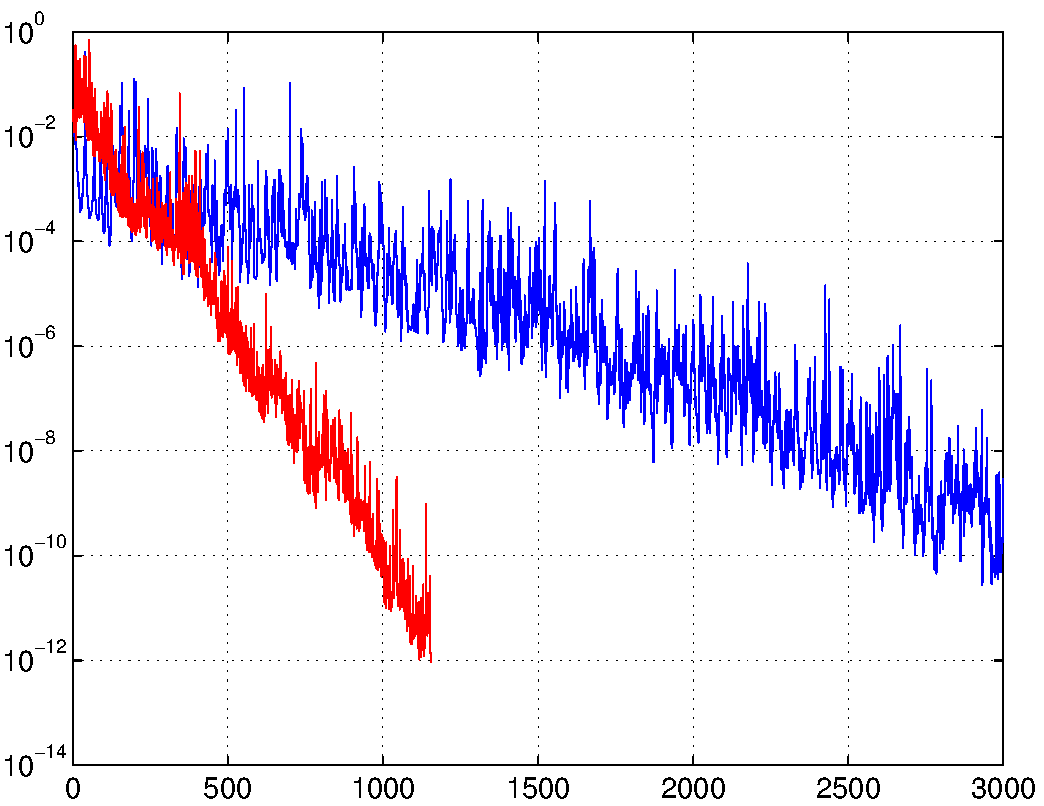
\includegraphics[width=.5\textwidth]{figures/cmg/history_grid3_newton1}}
  \subfigure[2nd Newton step]{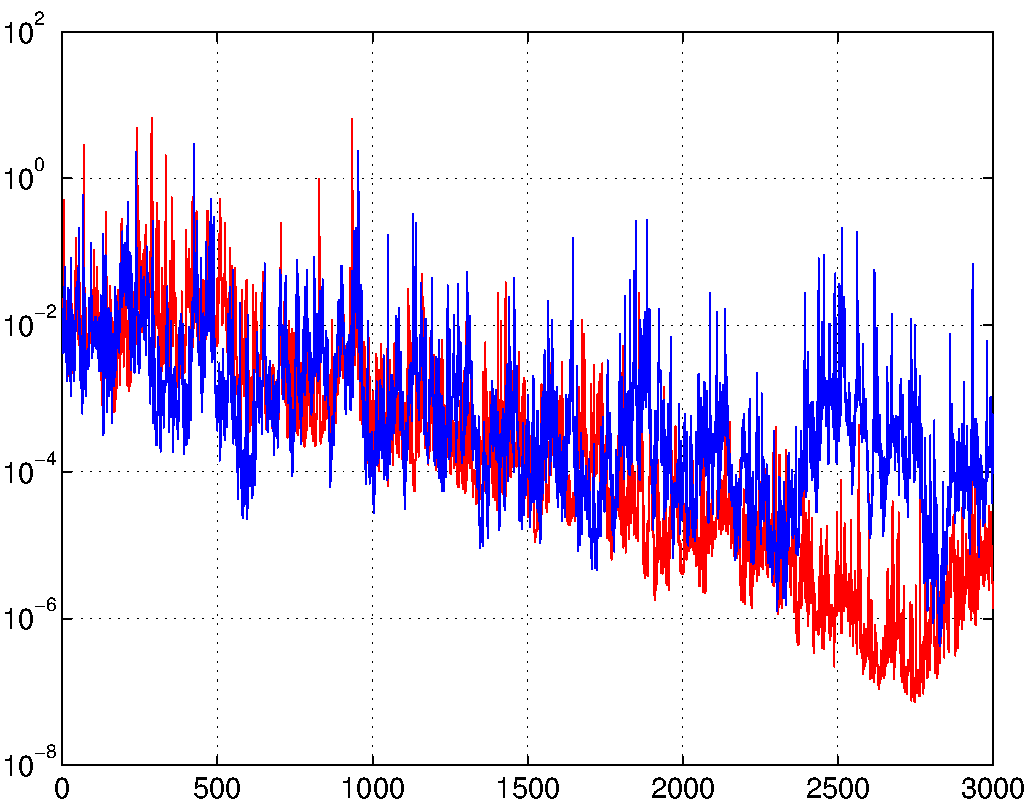
\includegraphics[width=.5\textwidth]{figures/cmg/history_grid3_newton2_a}}
  \caption{Convergence histories for different scalings of the pressure block}
  \label{fig:precond}
\end{figure}
%

\subsection{Application Studies}

% \subsubsection{Rayleigh-B\'enard-Maragoni flow} \label{RBMFlow}
% In this subsection we consider the steady state fluid-thermal
% problem (\ref{momentum_algb_eqn})-(\ref{thermal_algb_eqn}) in the
% unit cube. In this study with non-dimensional variables, the
% bottom wall is held at $T=350$ and the top wall is held at $T=300$.
% The zero slip boundary condition is imposed on the bottom and top
% walls, and on two opposite side walls. The constant tangential
% slip boundary condition $(0,100,0)$ is imposed on one of the others
% walls. The other boundary conditions are natural. 

% Table~\ref{table_RBM} collates results of numerical experiments with the CMG on a
% sequence of 4 uniformly refined grids and without it. Both methods
% are started with zero initial guesses which are refined
% during 6 Newton iterations using the BCG method.
% The stopping criterion for BCG iterations was
% the relative decrease of $L_2$ norm of the initial residual in $10^8$
% times for the 1st grid and $10^4$ for the others.

% Since the problem size is increased approximately 8 times during
% the refinement process, the computations on the final grid are 
% most time consuming. Table~\ref{table_RBM} shows the excelent performance of
% the CMG method. Despite the problem nonlinearity the number of
% smoothing iterates is rapidly decreased on finer grids.


% \begin{table}[hbt]

%     \begin{centering}

%         \caption{Number of BCG sweeps for the fluid-thermal problem.}
%         \label{table_RBM}
%         \vspace{1ex}

%         \begin{tabular}{rrrr|r}
%             \hline
%             \multicolumn{4}{c|}{Cascadic MG} & no CMG \\[.5ex]
%             \hline
%             1st grid & 2nd grid & 3rd grid & 4th grid & 4th grid
% \\[.5ex]
%             \hline
%             111 & 1206 & 90 & 41 &  114~ \\[.5ex]
%             512 &  376 & 27 &  1 & 3000* \\[.5ex]
%             407 &   19 &  1 &  3 &  632~ \\[.5ex]
%             260 &    1 &  1 &  1 &  502~ \\[.5ex]
%             4 &    1 &  1 &  1   &   11~ \\[.5ex]
%             1 &    1 &  1 &  6   &    3~ \\[.5ex]
%         \end{tabular}

%     \end{centering}

% \end{table}



\subsubsection{3D Lid-Driven Cavity}
In this subsection we consider the three-dimensional, incompressible flow of a lid-driven cavity.  The Reynolds number for this case is 100.  No-slip is imposed on the bottom and four sides of the unit cube domain, while the top is a free surface with $\bu$ specified to drive the system.  The problem is solved on 8 processors of a PC cluster. Isobars of pressure and streamlines are shown on a half domain cross section in Figure~\ref{fig:3D_cavity}.  In the Figure the red lines denote subdomain boundaries. On the top surface flow is in the direction of the $x$-axis.

\begin{figure}[hbtp]
  \begin{center}
    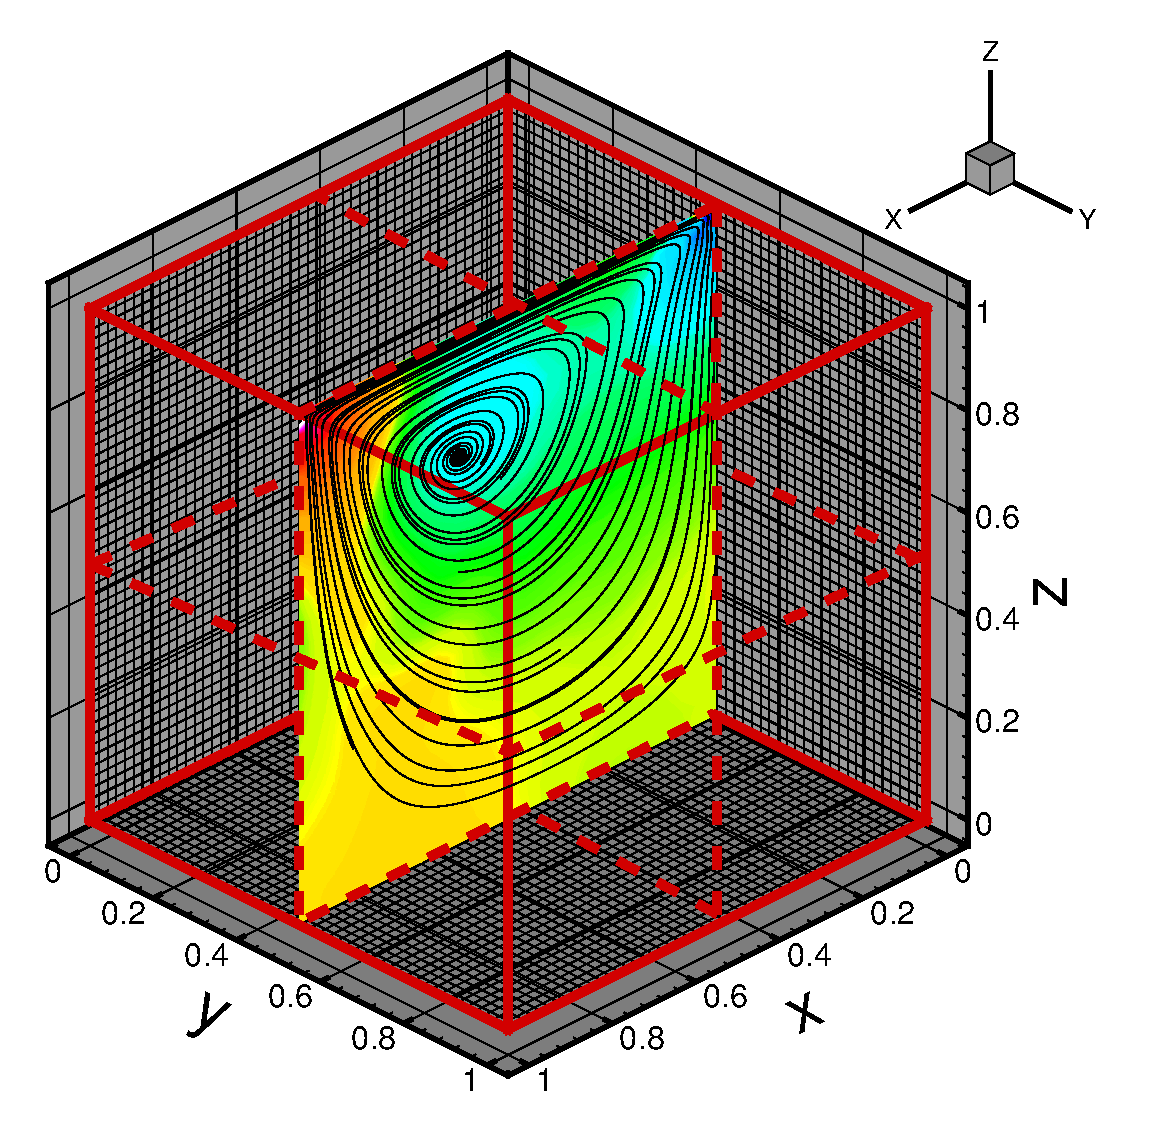
\includegraphics[width=.6\textwidth]{figures/cmg/flowfield-3D}
    \caption{Pressure isobars and streamlines for a driven cavity at $Re=100$.}
    \label{fig:3D_cavity}
  \end{center}
\end{figure}
    

\begin{table}[hbtp]

    \begin{centering}

        \caption{Total Number of BCG sweeps for the 3D NS problem, $\epsilon=10^{-5}$}
        \label{table_3D_1}
        \vspace{1ex}

        \begin{tabular}{|l|rrrr|} \hline

                     & \multicolumn{4}{c|}{Grid Size}                  \\
            
                     & $6\times  6\times  6$  & $12\times 12 \times 12$ 
                     & $24\times 24\times 24$ & $48\times 48 \times 48$ \\ \hline
        CMG          & 905      & 1366       & 2808       &  6888      \\ 
        No MG        & 905      & 1406       & 2909       &  8060      \\ \hline
        Work Ratio   & 1        & 0.97       & 0.97       &  0.85      \\ \hline
        
        \end{tabular}

    \end{centering}

\end{table}
\begin{table}[hbtp]

    \begin{centering}

        \caption{Total Number of BCG sweeps for the 3D NS problem, $\epsilon=10^{-6}$}
        \label{table_3D_2}
        \vspace{1ex}

        \begin{tabular}{|l|rrrr|} \hline

                     & \multicolumn{4}{c|}{Grid Size}                  \\
            
                     & $6\times  6\times  6$  & $12\times 12\times 12$ 
                     & $24\times 24\times 24$ & $48\times 48\times 48$ \\ \hline
         CMG         & 905      &  2275      &  5212      & 9913       \\
         No MG       & 905      &  2013      &  4853      & 12625      \\ \hline
         Work Ratio  & 1        &  1.13      &  1.07      & 0.79       \\ \hline
        
        \end{tabular}

    \end{centering}

\end{table}



Tables \ref{table_3D_1} and \ref{table_3D_2} show results of the numerical experiment for two different BCG stopping criteria with CMG applied to a sequence of 4 uniformly refined grids, and the same grid sequence without CMG.  The number of BCG iterations required for the 5 Newton steps is summed and tabulated.  For this sequence the first grid was composed of $6\times 6 \times 6=216$ elements, 
while the last grid contained $48\times 48\times 48=110,592$ elements. 
For all cases the initial coarse grid problem was solved to a tolerance of $\epsilon=10^{-6}$ (measured as relative decrease of the $L_2$ norm of the residual). In Table~\ref{table_3D_1} the remainder of the simulations were solved to a tolerance of $\epsilon=10^{-5}$, and in Table~\ref{table_3D_2} the tolerance $\epsilon=10^{-6}$ was used.

The tables do not allow for a definite conclusion with regard to the performance of the method.  In the first case it is apparent that 15\% less work was required on the final grid, and that less work was required at each intermiediate step when the CMG algorithm was applied.  Additionally, in the second experiment it is apparent that 21\% less work was required on the finest mesh considered.  This is a reasonable performance increase, particularly when considering how easily the algorithm was implemented into the existing code.  However, at two intermediate steps the CMG approach actually required \emph{more} work than the straightforward approach.  This numerical experiment does not allow us to make any definite conclusions about the error behavior on the sequence of successively refined grids.



\subsubsection{2D Lid-Driven Cavity}
In this subsection we continue the previous experiment in 2D and examine the effect of different iterative solvers on the performance of the CMG algorithm.  Again, the application of interest is a lid-driven cavity containing an incompressible fluid at Reynolds number of~100. Isobars and streamlines are shown for the steady solution in Figure~\ref{fig:2D}.

For this case three different iterative solvers were employed: bi-conjugate gradient (BCG), bi-conjugate gradient stabilized (BCG-Stab), and the generalized-minimum residual method with 50 search vectors (GMRES-50).  In all cases the linear system was preconditioned with Jacobi (diagonal) preconditioning.
\begin{figure}[hbt]
  \begin{center}
    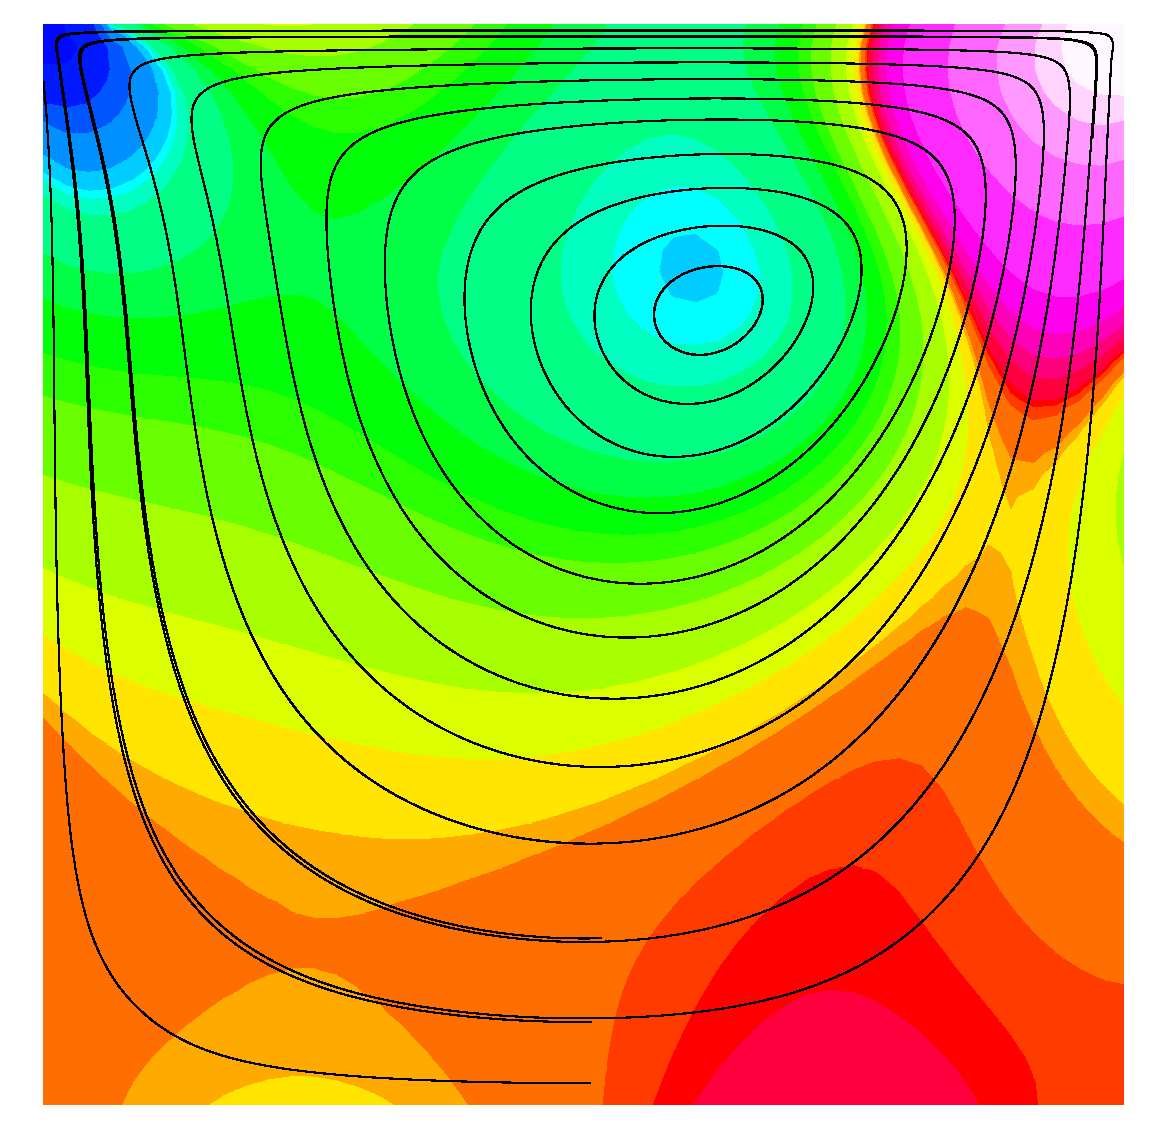
\includegraphics[width=.4\textwidth]{figures/cmg/flowfield-2D}
    \caption{Pressure contours and streamlines for a driven cavity at $Re=100$.}
    \label{fig:2D}
  \end{center}
\end{figure}


Tables~\ref{table:2D_1}-\ref{table:2D_3} show results of the numerical experiment with each iterative solver.  Note that in each case a stopping criterion of $\epsilon=10^{-5}$ (measured as relative decrease of the $L_2$ norm of the residual) was used.

In this experiment it is obvious that the most benefit was achieved from CMG when using the GMRES algorithm.  The least benefit was obtained when using BCG.  In analyzing these results it is useful to examine the behavior of the individual algorithms. Figure~\ref{fig:resid_hist} shows the residual history on the finest mesh for the three different iterative solvers. The figure corresponds to the finest mesh in the case of CMG.
    
    \begin{table}[hbt]

        \begin{centering}
        
        \caption{Total Number of BCG sweeps for the 2D NS problem}
        \label{table:2D_1}
        \vspace{1ex}
        \begin{tabular}{|l|rrrr|} \hline
                    & \multicolumn{4}{c|}{Grid Size}                  \\
                    & $6\times 6$ & $12\times 12$ 
                    & $24\times 24$ & $48\times 48$ \\ \hline
        CMG         & 448   &  952    & 1767    & 6875    \\ 
        No MG       & 448   &  1157   & 2940    & 11124   \\ \hline
        Work Ratio  & 1     &  0.82   & 0.60    & 0.62    \\ \hline
      \end{tabular}

      \end{centering}
    
    \end{table}
    \begin{table}[hbt]

        \begin{centering}
        
        \caption{Total Number of BCG--Stab sweeps for the 2D NS problem}
        \label{table:2D_2}
        \vspace{1ex}
        \begin{tabular}{|l|rrrr|} \hline
                    & \multicolumn{4}{c|}{Grid Size}                  \\
                    & $6\times 6$ & $12\times 12$ 
                    & $24\times 24$ & $48\times 48$ \\ \hline
        CMG         & 513 & 757       & 1663    & 2513    \\ 
        No MG       & 513 & 1056      & 2571    & 6154    \\ \hline
        Work Ratio  & 1   & 0.72      & 0.65    & 0.41    \\ \hline    
        \end{tabular}

        \end{centering}

    \end{table}        
    \begin{table}[hbt]

        \begin{centering}
        
        \caption{Total Number of GMRES--50 sweeps for the 2D NS problem}
        \label{table:2D_3}
        \vspace{1ex}
        \begin{tabular}{|l|rrrr|} \hline
                    & \multicolumn{4}{c|}{Grid Size}                  \\
                    & $6\times 6$ & $12\times 12$ 
                    & $24\times 24$ & $48\times 48$ \\ \hline
        CMG         & 681   & 1261    & 2442    & 5696    \\ 
        No MG       & 681   & 1657    & 4719    & 17678   \\ \hline
        Work Ratio  & 1     & 0.76    & 0.52    & 0.32    \\ \hline    
        \end{tabular}

        \end{centering}

    \end{table}

    
It is apparent from the figure that the three methods behave quite differently.  Both BCG and BCG-Stab are erratic.  Of these two methods BCG-Stab behaves better in the sense that it consistently achieves smaller residuals than BCG.  In fact, for much of the computation the residual obtained with BCG is \emph{two orders of magnitude higher} than the initial residual.  Since the initial solution is fairly close to the correct solution in this case BCG is particularly ill-suited for use in the CMG algorithm.

\begin{figure}
  \begin{center}
    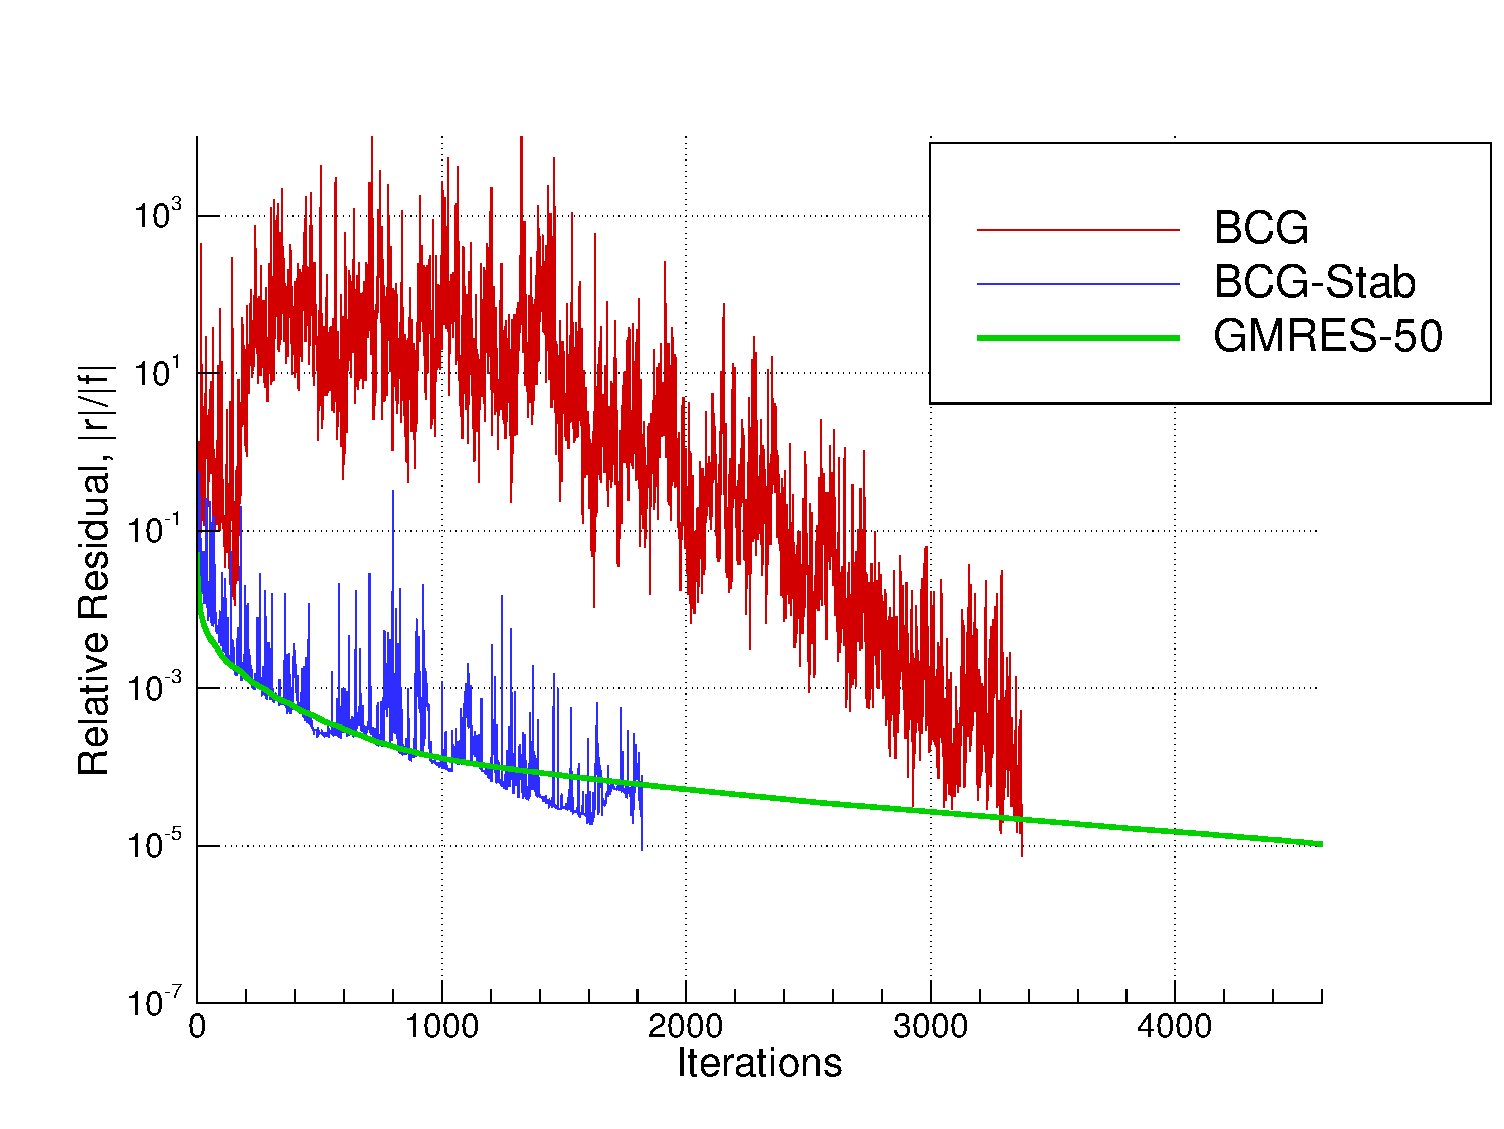
\includegraphics[width=.85\textwidth]{figures/cmg/history_bcg_bcgstab_gmres}
    \caption{Relative Residual History for the 2D Experiment}
    \label{fig:resid_hist}
  \end{center}
\end{figure}

Conversely, GMRES behaves monotonically.  The initial solution is close to the exact solution, and at each step of the algorithm the residual is reduced.  This behavior is much like that of the conjugate-gradient algorithm and symmetric systems for which the CMG method was originally derived.  The optimality of the method that was presented earlier (in Section~\ref{cmg_theory}) was based on the fundamental assumption that each sweep of the iterative solver reduced the error in the linear system, and thus it is not surprising that GMRES converges significantly faster in the context of CMG.

From this numerical experiment it is apparent that CMG can provide a significant speedup even for problems with convection when used in applications that employ GMRES, CG, or some relaxation method to solve linear systems.  For other, less predictable algorithms (such as BCG and BCG-Stab) the benefit of the CMG method is not entirely clear.


%%%%%%%%%%%%%%%%%%%%%%%%%%%%%%%%%%%%%%%%%%%%%%%%%%%%%%%%%%%
\section{Concluding Remarks}
The cascadic multigrid approach (CMG) has been discussed and applied to incompressible flow transport problems.  The scheme is found to provide optimal arithmetic complexity in 3D when the conjugate gradient (CG) iterative scheme is used as a smoother at each grid level.  Numerical experiments suggest that this optimality can be maintained in the case of nonlinear, non-symmetric problems provided that the smoother has CG-like properties.  Accordingly, little benefit was gained from CMG when BCG or BCG-Stab were used as grid smoothers (whose convergence properties bear little resemblance to CG), while appreciable benefit was gained from CMG when GMRES was used as the smoother.  This is behavior is likely due to the fact that GMRES's monotonic convergence properties fit within the CMG theoretical assumptions. 


%% Local Variables:
%% TeX-master: "dissertation.tex"
%% End:
